\documentclass{ximera}

%\usepackage{todonotes}

\newcommand{\todo}{}

\usepackage{esint} % for \oiint
\ifxake%%https://math.meta.stackexchange.com/questions/9973/how-do-you-render-a-closed-surface-double-integral
\renewcommand{\oiint}{{\large\bigcirc}\kern-1.56em\iint}
\fi


\graphicspath{
  {./}
  {ximeraTutorial/}
  {basicPhilosophy/}
  {functionsOfSeveralVariables/}
  {normalVectors/}
  {lagrangeMultipliers/}
  {vectorFields/}
  {greensTheorem/}
  {shapeOfThingsToCome/}
  {dotProducts/}
  {partialDerivativesAndTheGradientVector/}
  {../productAndQuotientRules/exercises/}
  {../normalVectors/exercisesParametricPlots/}
  {../continuityOfFunctionsOfSeveralVariables/exercises/}
  {../partialDerivativesAndTheGradientVector/exercises/}
  {../directionalDerivativeAndChainRule/exercises/}
  {../commonCoordinates/exercisesCylindricalCoordinates/}
  {../commonCoordinates/exercisesSphericalCoordinates/}
  {../greensTheorem/exercisesCurlAndLineIntegrals/}
  {../greensTheorem/exercisesDivergenceAndLineIntegrals/}
  {../shapeOfThingsToCome/exercisesDivergenceTheorem/}
  {../greensTheorem/}
  {../shapeOfThingsToCome/}
  {../separableDifferentialEquations/exercises/}
  {vectorFields/}
}

\newcommand{\mooculus}{\textsf{\textbf{MOOC}\textnormal{\textsf{ULUS}}}}

\usepackage{tkz-euclide}
\usepackage{tikz}
\usepackage{tikz-cd}
\usetikzlibrary{arrows}
\tikzset{>=stealth,commutative diagrams/.cd,
  arrow style=tikz,diagrams={>=stealth}} %% cool arrow head
\tikzset{shorten <>/.style={ shorten >=#1, shorten <=#1 } } %% allows shorter vectors

\usetikzlibrary{backgrounds} %% for boxes around graphs
\usetikzlibrary{shapes,positioning}  %% Clouds and stars
\usetikzlibrary{matrix} %% for matrix
\usepgfplotslibrary{polar} %% for polar plots
\usepgfplotslibrary{fillbetween} %% to shade area between curves in TikZ
%\usetkzobj{all}
\usepackage[makeroom]{cancel} %% for strike outs
%\usepackage{mathtools} %% for pretty underbrace % Breaks Ximera
%\usepackage{multicol}
\usepackage{pgffor} %% required for integral for loops



%% http://tex.stackexchange.com/questions/66490/drawing-a-tikz-arc-specifying-the-center
%% Draws beach ball
\tikzset{pics/carc/.style args={#1:#2:#3}{code={\draw[pic actions] (#1:#3) arc(#1:#2:#3);}}}



\usepackage{array}
\setlength{\extrarowheight}{+.1cm}
\newdimen\digitwidth
\settowidth\digitwidth{9}
\def\divrule#1#2{
\noalign{\moveright#1\digitwidth
\vbox{\hrule width#2\digitwidth}}}




% \newcommand{\RR}{\mathbb R}
% \newcommand{\R}{\mathbb R}
% \newcommand{\N}{\mathbb N}
% \newcommand{\Z}{\mathbb Z}

\newcommand{\sagemath}{\textsf{SageMath}}


%\renewcommand{\d}{\,d\!}
%\renewcommand{\d}{\mathop{}\!d}
%\newcommand{\dd}[2][]{\frac{\d #1}{\d #2}}
%\newcommand{\pp}[2][]{\frac{\partial #1}{\partial #2}}
% \renewcommand{\l}{\ell}
%\newcommand{\ddx}{\frac{d}{\d x}}

% \newcommand{\zeroOverZero}{\ensuremath{\boldsymbol{\tfrac{0}{0}}}}
%\newcommand{\inftyOverInfty}{\ensuremath{\boldsymbol{\tfrac{\infty}{\infty}}}}
%\newcommand{\zeroOverInfty}{\ensuremath{\boldsymbol{\tfrac{0}{\infty}}}}
%\newcommand{\zeroTimesInfty}{\ensuremath{\small\boldsymbol{0\cdot \infty}}}
%\newcommand{\inftyMinusInfty}{\ensuremath{\small\boldsymbol{\infty - \infty}}}
%\newcommand{\oneToInfty}{\ensuremath{\boldsymbol{1^\infty}}}
%\newcommand{\zeroToZero}{\ensuremath{\boldsymbol{0^0}}}
%\newcommand{\inftyToZero}{\ensuremath{\boldsymbol{\infty^0}}}



% \newcommand{\numOverZero}{\ensuremath{\boldsymbol{\tfrac{\#}{0}}}}
% \newcommand{\dfn}{\textbf}
% \newcommand{\unit}{\,\mathrm}
% \newcommand{\unit}{\mathop{}\!\mathrm}
% \newcommand{\eval}[1]{\bigg[ #1 \bigg]}
% \newcommand{\seq}[1]{\left( #1 \right)}
% \renewcommand{\epsilon}{\varepsilon}
% \renewcommand{\phi}{\varphi}


% \renewcommand{\iff}{\Leftrightarrow}

% \DeclareMathOperator{\arccot}{arccot}
% \DeclareMathOperator{\arcsec}{arcsec}
% \DeclareMathOperator{\arccsc}{arccsc}
% \DeclareMathOperator{\si}{Si}
% \DeclareMathOperator{\scal}{scal}
% \DeclareMathOperator{\sign}{sign}


%% \newcommand{\tightoverset}[2]{% for arrow vec
%%   \mathop{#2}\limits^{\vbox to -.5ex{\kern-0.75ex\hbox{$#1$}\vss}}}
% \newcommand{\arrowvec}[1]{{\overset{\rightharpoonup}{#1}}}
% \renewcommand{\vec}[1]{\arrowvec{\mathbf{#1}}}
% \renewcommand{\vec}[1]{{\overset{\boldsymbol{\rightharpoonup}}{\mathbf{#1}}}}

% \newcommand{\point}[1]{\left(#1\right)} %this allows \vector{ to be changed to \vector{ with a quick find and replace
% \newcommand{\pt}[1]{\mathbf{#1}} %this allows \vec{ to be changed to \vec{ with a quick find and replace
% \newcommand{\Lim}[2]{\lim_{\point{#1} \to \point{#2}}} %Bart, I changed this to point since I want to use it.  It runs through both of the exercise and exerciseE files in limits section, which is why it was in each document to start with.

% \DeclareMathOperator{\proj}{\mathbf{proj}}
% \newcommand{\veci}{{\boldsymbol{\hat{\imath}}}}
% \newcommand{\vecj}{{\boldsymbol{\hat{\jmath}}}}
% \newcommand{\veck}{{\boldsymbol{\hat{k}}}}
% \newcommand{\vecl}{\vec{\boldsymbol{\l}}}
% \newcommand{\uvec}[1]{\mathbf{\hat{#1}}}
% \newcommand{\utan}{\mathbf{\hat{t}}}
% \newcommand{\unormal}{\mathbf{\hat{n}}}
% \newcommand{\ubinormal}{\mathbf{\hat{b}}}

% \newcommand{\dotp}{\bullet}
% \newcommand{\cross}{\boldsymbol\times}
% \newcommand{\grad}{\boldsymbol\nabla}
% \newcommand{\divergence}{\grad\dotp}
% \newcommand{\curl}{\grad\cross}
%\DeclareMathOperator{\divergence}{divergence}
%\DeclareMathOperator{\curl}[1]{\grad\cross #1}
% \newcommand{\lto}{\mathop{\longrightarrow\,}\limits}

% \renewcommand{\bar}{\overline}

\colorlet{textColor}{black}
\colorlet{background}{white}
\colorlet{penColor}{blue!50!black} % Color of a curve in a plot
\colorlet{penColor2}{red!50!black}% Color of a curve in a plot
\colorlet{penColor3}{red!50!blue} % Color of a curve in a plot
\colorlet{penColor4}{green!50!black} % Color of a curve in a plot
\colorlet{penColor5}{orange!80!black} % Color of a curve in a plot
\colorlet{penColor6}{yellow!70!black} % Color of a curve in a plot
\colorlet{fill1}{penColor!20} % Color of fill in a plot
\colorlet{fill2}{penColor2!20} % Color of fill in a plot
\colorlet{fillp}{fill1} % Color of positive area
\colorlet{filln}{penColor2!20} % Color of negative area
\colorlet{fill3}{penColor3!20} % Fill
\colorlet{fill4}{penColor4!20} % Fill
\colorlet{fill5}{penColor5!20} % Fill
\colorlet{gridColor}{gray!50} % Color of grid in a plot

\newcommand{\surfaceColor}{violet}
\newcommand{\surfaceColorTwo}{redyellow}
\newcommand{\sliceColor}{greenyellow}




\pgfmathdeclarefunction{gauss}{2}{% gives gaussian
  \pgfmathparse{1/(#2*sqrt(2*pi))*exp(-((x-#1)^2)/(2*#2^2))}%
}


%%%%%%%%%%%%%
%% Vectors
%%%%%%%%%%%%%

%% Simple horiz vectors
\renewcommand{\vector}[1]{\left\langle #1\right\rangle}


%% %% Complex Horiz Vectors with angle brackets
%% \makeatletter
%% \renewcommand{\vector}[2][ , ]{\left\langle%
%%   \def\nextitem{\def\nextitem{#1}}%
%%   \@for \el:=#2\do{\nextitem\el}\right\rangle%
%% }
%% \makeatother

%% %% Vertical Vectors
%% \def\vector#1{\begin{bmatrix}\vecListA#1,,\end{bmatrix}}
%% \def\vecListA#1,{\if,#1,\else #1\cr \expandafter \vecListA \fi}

%%%%%%%%%%%%%
%% End of vectors
%%%%%%%%%%%%%

%\newcommand{\fullwidth}{}
%\newcommand{\normalwidth}{}



%% makes a snazzy t-chart for evaluating functions
%\newenvironment{tchart}{\rowcolors{2}{}{background!90!textColor}\array}{\endarray}

%%This is to help with formatting on future title pages.
\newenvironment{sectionOutcomes}{}{}



%% Flowchart stuff
%\tikzstyle{startstop} = [rectangle, rounded corners, minimum width=3cm, minimum height=1cm,text centered, draw=black]
%\tikzstyle{question} = [rectangle, minimum width=3cm, minimum height=1cm, text centered, draw=black]
%\tikzstyle{decision} = [trapezium, trapezium left angle=70, trapezium right angle=110, minimum width=3cm, minimum height=1cm, text centered, draw=black]
%\tikzstyle{question} = [rectangle, rounded corners, minimum width=3cm, minimum height=1cm,text centered, draw=black]
%\tikzstyle{process} = [rectangle, minimum width=3cm, minimum height=1cm, text centered, draw=black]
%\tikzstyle{decision} = [trapezium, trapezium left angle=70, trapezium right angle=110, minimum width=3cm, minimum height=1cm, text centered, draw=black]


\title{Analyzing}

\begin{document}

\begin{abstract}
describe everything
\end{abstract}
\maketitle



$\blacktriangleright$ \textbf{\textcolor{red!80!black}{Reasoning:}} Reasoning is a logical explanation that describes our conclusions, how we arrived at those conclusions, and why we think those conclusions are correct. \\

Analysis is not a list of conclusions. We are not looking for such a list. \\

We are looking for the thought process that arrived at the list of conclusions. \\








\begin{example}

\textbf{\textcolor{purple!85!blue}{Completely analyze $K(x) = \ln(x^2+2x+3)$}} \\



\textbf{\textcolor{blue!55!black}{$\blacktriangleright$ Domain}}  $K$ is a composition of a logarithm function and a quadratic function. 


$K(x) = (outside \circ inside)(x) = outside(inside(x))$ where


\begin{itemize}
\item $outside(y) = \ln(y)$ with natural domain  $(0, \infty)$ \\
\item $inside(v) = v^2 + 2v + 3$ with natural domain $(-\infty, \infty)$
\end{itemize}


We need the range of $inside$ to be inside the domain of $outside$.\\

Therefore, domain of $K$ is all real numbers that make the inside function, $inside(v)=v^2+2v+3$, greater than $0$.  So, we need some information about $inside(v)=v^2+2v+3$.  \\  


$inside(v)$ is a \wordChoice{\choice{linear} \choice{radical} \choice[correct]{quadratic} \choice{rational}}  function.  Its leading coefficient is \wordChoice{\choice[correct]{positive} \choice{negative}}. \\


A quadratic function with a postive leading tells us that $inside(v)$ has an absolute \wordChoice{\choice{maximum} \choice[correct]{minimum}}.  The quadratic formula tells us that the minimum occurs at $v=\frac{-b}{2a} = \frac{\answer{-2}}{\answer{2}} = -1$. \\

The minimum value of $inside(v)$ is $inside(-1) = \answer{2}$.  \\

Therefore, $inside(v) > 0$ for all $v$. Therefore, all values of $inside(v)$ are in the domain of the natural logarithm. \\

Therefore, the natural or implied domain of $K(x)$ is all real numbers, $(-\infty, \infty)$. \\









\textbf{\textcolor{blue!55!black}{$\blacktriangleright$ Zeros}} 


$outside(y) = \ln(y)$ is a logarithmic function, whose zero is $1$. \\

We need to find where $inside(v) = 1$. We just saw that $inside(v)$ is a quadratic function with a minimum value of $2$.  $inside(v)$ never equals $1$.  $K$ has no zeros. \\






\textbf{\textcolor{blue!55!black}{$\blacktriangleright$ Continuity}} 


Quadratic and logarithmic functions are both continuous. So, their composition is continuous. \\




\textbf{\textcolor{blue!55!black}{$\blacktriangleright$ End Behavior}} 






$\blacktriangleright$ Since $inside(v) = v^2 + 2v + 3$ is a quadratic with postive leading coefficient, we know that 
\[  \lim\limits_{v \to \infty}inside(v) = \answer{\infty}  \, \text{ and } \,  \lim\limits_{v \to -\infty}inside(v) = \answer{\infty}  \]


The end-behavior of $K$ is the end-behavior of $outside(y)$ with $y$ approaching $\infty $. \\



\[  
\lim\limits_{x \to -\infty}K(x) =  \lim\limits_{y \to \infty}outside(y) =   \lim\limits_{y \to \infty}\ln(y) =  \answer{\infty}
\]





\[  
\lim\limits_{x \to \infty}K(x) =  \lim\limits_{y \to \infty}outside(y) =   \lim\limits_{y \to \infty}\ln(y) =  \answer{\infty}
\]












\textbf{\textcolor{blue!55!black}{$\blacktriangleright$ Behavior}} 


$K$ is a composition, so we need the behavior of each component function. \\




$inside(v) = v^2 + 2v + 3$ is a quadratic function with a positive leading coefficient, which means it decreases and then increases, switching at its critical number of $-1$. \\

\begin{itemize}
\item $inside(v)$ decreases on $(-\infty, -1)$ \\
\item $inside(v)$ increases on $(-1, \infty)$ 
\end{itemize}




$outside(y) = \ln(y)$ is a logarithmic function with a positive leading coefficient whose inner linear function also has a positive leading coefficient. That tell us that $outside$ is always increasing. \\


On $\left( -\infty, \answer{-1} \right)$, $K = increasing \circ decreasing = decreasing$\\


On $\left( \answer{-1}, \infty \right)$, $K = increasing \circ increasing = increasing$\\









\textbf{\textcolor{blue!55!black}{$\blacktriangleright$ Local Maximums and Minimums}} 


$K$ is continuous.  It decreases and then increases giving it one critical number, which must be the location of a global minimum value, which is automatically a local minimum. \\

$K$ has a local minimum value of $K$ is $K(-1) = \ln(2)$. \\


There are no other critical numbers, so $K$ has no local maximum values. \\






\textbf{\textcolor{blue!55!black}{$\blacktriangleright$ Global Maximums and Minimums}} 


$K$ has a global minimum value of $K$ is $K(-1) = \ln(2)$, since it is continuous with only one local minimum value. \\




Since $\lim\limits_{x \to \infty}K(x) = \infty$, $K$ has no global maximum value.












\textbf{\textcolor{blue!55!black}{$\blacktriangleright$ Range}} 


$K$ is continuous. \\

$\lim\limits_{x \to \infty}K(x) = \infty$ \\

The global minimum value of $K$ is $\ln(2)$. \\



That give a range of  $[ \ln(2), \infty )$








This all agrees with the graph.






\begin{image}
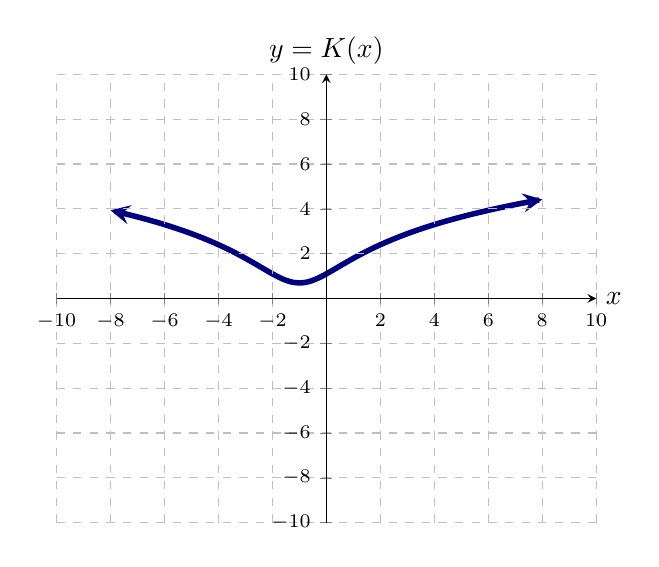
\begin{tikzpicture}
  \begin{axis}[
            domain=-10:10, ymax=10, xmax=10, ymin=-10, xmin=-10,
            axis lines =center, xlabel=$x$, ylabel={$y=K(x)$}, grid = major, grid style={dashed},
            ytick={-10,-8,-6,-4,-2,2,4,6,8,10},
            xtick={-10,-8,-6,-4,-2,2,4,6,8,10},
            yticklabels={$-10$,$-8$,$-6$,$-4$,$-2$,$2$,$4$,$6$,$8$,$10$}, 
            xticklabels={$-10$,$-8$,$-6$,$-4$,$-2$,$2$,$4$,$6$,$8$,$10$},
            ticklabel style={font=\scriptsize},
            every axis y label/.style={at=(current axis.above origin),anchor=south},
            every axis x label/.style={at=(current axis.right of origin),anchor=west},
            axis on top
          ]
          
          %\addplot [line width=2, penColor2, smooth,samples=100,domain=(-6:2)] {-2*x-3};
          \addplot [line width=2, penColor, smooth,samples=100,domain=(-8:8),<->] {ln(x^2 + 2*x + 3)};

  \end{axis}
\end{tikzpicture}
\end{image}







\end{example}










\subsection*{with Calculus}

\textbf{\textcolor{red!70!black}{A Peek Ahead...}}


Calculus will give us the derivative: $K'(x) = \frac{2x+2}{x^2+2x+3}$.  We could then solve $K'(x) = 0$ and get $x=-1$ as the only critical number, which agrees with what we found. \\



We showed above that $x^2+2x+3$ was a positive function.  So, the sign of $K'(x)$ is the same as the sign of $2x+2$. \\

$2x+2$ is a linear funciton with a positive leading coefficient.  Therefore, it is negative on $(-\infty, -1)$  and positive on $(-1, \infty)$. \\


$K$ is decreasing on $(-\infty, -1)$ and increasing on $(-1, \infty)$.











\begin{center}
\textbf{\textcolor{green!50!black}{ooooo-=-=-=-ooOoo-=-=-=-ooooo}} \\

more examples can be found by following this link\\ \link[More Examples of Analyzing Functions]{https://ximera.osu.edu/csccmathematics/precalculus2/precalculus2/analyzingFunctions/examples/exampleList}

\end{center}







\end{document}
